\chapter{Architecture}\label{chp-arch}
\section{Overview}
Labrador was designed from the ground up as a distributed crawler. As such, its code base consists of two major programs, the Dispatcher and the Crawlers, with some shared components. This chapter describes the architecture of each of those components and the distributed techniqueues used to increase the crawl speed.
\subsection{Dispatcher}
The dispatcher is responsible for co-ordinating the crawlers, as the crawlers do not directly interact among themselves. Essentially this amounts to four primary tasks:
\begin{itemize}
\item{Informing crawlers of their configuration.}
\item{Allocating URLs to crawlers.}
\item{Managing shared data - robots.txt files and document fingerprints for duplicate detection.}
\item{Collecting and aggregating statistics concerning the crawl.}
\end{itemize}

\subsection{Crawlers}
Labrador's crawler processes are responsible for fetching, parsing and saving retrieved pages. Under normal circumstances Labrador has several crawlers running on a machine concurrently, permitting multiple fetches to be occuring concurrently and allowing the operating system to handle concurrency issues. URLs are extracted from the links on the pages during the parsing phase and handled by the current crawler Manager module, which may pass some or all back to the dispatcher. All URLs found are passed back to the dispatcher unless the crawler has been configured as a partitioned crawler and some of the links fall out-with the crawlers own partition. More information on partitioning of crawls can be found in Section \ref{sect-partitioning}.

\begin{figure}[h]
  \centerline{
    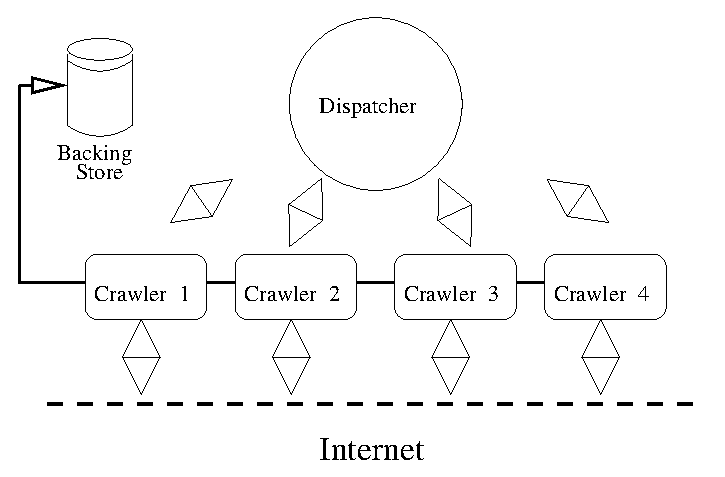
\epsfig{file=./images/crawler_overview.eps, scale=0.75}
  }
  \caption{Architecture Overview}
  \label{fig-architecture}
\end{figure}

\subsection{Implementation}
Labrador is implemented in Perl using object-oriented modules. Perl is not a common development language in this department, however it had several attributes that made it a good choice for writing a crawler:
\begin{itemize}
\item{Firstly, the Comprehensive Perl Archive Network\cite{site1} (CPAN) is the Perl language's open source repository of useful modules. Most modules in CPAN are very mature due to peer usage and review. The archive is very extensive in breadth of modules available. Examples of modules of which I made extensive use: HTML Link Extaction; URL Normalisation; HTTP Fetching; Robots.txt parsing.}
\item{The language's extensive string processing facilities, particularly Perl's regular expression engine.}
\item{Perl's low-level interface to the Unix system calls, which allow very direct manipulation of sockets.}
\item{Not least, my own familiarity with the language. This was massively beneficial, as well as the expressiveness of the language, which allows succinct coding of complex concepts.}
\end{itemize}

\section{Crawler - Dispatcher Communication}
Labrador was designed around minimising network traffic between the dispatcher and the crawlers. One TCP connection is opened between each crawler and the dispatcher. Crawlers ask `questions' to the dispatcher, which processes the question and then `answers' the crawler in an agreed protocol.

\subsection{Network Protocol}
The protocol was design to be easily human readable, while still easy to parse using simple string processing functions or regular expressions. Questions and answers follow the same format: the verbname and the first parameter; followed by optional parameters; the end of the question or answer is marked by a single period followed by a new line. This is shown below:
\renewcommand{\baselinestretch}{1.0}
\begin{verbatim}
VERBNAME argument1
argument2 
argument3
many arguments
last argument number x
.
\end{verbatim}
\renewcommand{\baselinestretch}{1.5}

In `answer' messages, VERBNAME is replaced by a status code from which the client can deduce whether the request was successful or not. Additionally, it is common for argument1 to be a textual description of the status code to allow easier human interpretation of the reply. To anyone familiar with common Internet protocols, it can be seen that Labrador's network communication protocol takes wisdom from several common protocols, mainly the HTTP and the SMTP protocols. The use of a textual protocol ensures that the developer can easily inspect the raw message and ascertain the meaning and content of the message. By using the uncommon character combination of `\textbackslash n.\textbackslash n' as an end marker, it was straightforward to match one message by performing a substitution regular expression, or more simply using a linear string search function to find the sequence. It should be noted that regular expression implementations use the stack heavily and it was found that a 6000 line message exceeds the environment's default stack limit, causing a segmentation fault. Hence, a linear search, such as Perl's index() function, tends to be far faster.\\
\ \\
In Labrador's network protocol, the end of message marker described above (`\textbackslash n.\textbackslash n') came from the end of DATA block in the SMTP protocol\cite{rfc821}. The readable verb names and status codes were inspired by the HTTP protocol\cite{rfc2616}. Verbs can only be called when the calling client has sufficient privilege. Table \ref{tbl-commands} shows the supported commands and their privilege levels, while more in-depth information on the protocol itself can be found in Appendix \ref{appndx-protocol}.


\subsection{Dispatcher Network-level Design}\label{sect-dispnetworkdesign}
I was keen for Labrador's dispatcher to be built as a single-threaded application. There were several reasons behind this: 
\begin{itemize}
\item{Perl's thread support has not yet matured to a level with which I was happy, in particular, not all modules from CPAN are yet thread-safe.}
\item{A single-threaded program can be kept more simple, as there would be no need for complex locking of data structures, ensuring responsiveness and thread-safety.} 
\end{itemize}
Hence, while many crawlers can be connected to the dispatcher simultaneously, the dispatcher can only process one question at a time. However, due to Labrador's typical modus operandi, in which the crawl is partitioned, means that the dispatcher is not a bottleneck of the crawl. Partitioning is further described in \ref{sect-partitioning}.\\
\ \\
It has been standard practice in Unix programs for many years to use `non-blocking sockets' when a process must manipulate multiple network sockets without blocking for reading or writing on any single socket. Non-blocking sockets is a series of system calls which prevent blocking when reading or writing a socket. I based my low-level network code (the Connections module) on the non-blocking sockets example from the Perl Cookbook\cite{book1} (Recipe 17.13). A continuous loop is executed, which polls sockets for new incoming data, processes messages once a whole message has been received and sends as much data on a socket as possible without blocking. I had a problem with the Cookbook's handling of partial sends, so further referred to Unix Networking Programming\cite{book2} to fully understand the system calls involved. It is interesting that the Unix system call interface has changed so little in the last fourteen years, that the first edition was still relevant and that Perl's low-level treatment of sockets is so close to the actual system calls, that example networking source code can easily be migrated from C to Perl.

\subsection{Dispatcher Event Handling}\label{sect-dispevents}
The dispatcher is built on a layered architecture, which can be seen in Figure \ref{fig-disp_events}. The Connections module responsible for the network I/O as described in Section \ref{sect-dispnetworkdesign}, passing events up to the Events module. The Events module handles three primary events: crawler\_connect; crawler\_disconnection; and event\_command. The events module will inform the dispatcher directly of connections and disconnections. However, on a command invocation, the Events module will check to see if the Commands module has registered a command of that name, and if the crawler is privileged enough to execute the command. Different commands require different privilege levels, which is designed to ensure that only clients that are permitted to can peform certain commands. For instance, the dispatcher will not allow a crawl to be stopped unless the client had logged on using the correct administrator privilege password. All protocol commands and their privileges can be seen in Table \ref{tbl-commands}.\\
\begin{table}
\begin{center}
\begin{tabular}{|l|l|}
\hline
\bf{Command Name} & \bf{Privilege Level} \\
\hline
HELO & Any \\
\hline
QUIT & Any \\
\hline
NOOP & Any \\
\hline
CONF & Logged on \\
\hline
MONITOR & Logged on \\
\hline
WORK & Logged on \\
\hline
NEXT & Crawler \\
\hline
FINISHED & Crawler \\
\hline
FAILED & Crawler \\
\hline
ROBOTS & Crawler \\
\hline
ROBOTSFILE & Crawler \\
\hline
STATS & Crawler \\
\hline
FINGERPRINT & Crawler \\
\hline
SHUTDOWN & Crawler \\
\hline
ALLOWED & Crawler \\
\hline
CHECKPOINT & Administrator \\
\hline
PAUSE & Administrator \\
\hline
START & Administrator \\
\hline
STOP & Administrator \\
\hline
\end{tabular}
\caption{Network Protocol - Commands \& Privileges. Further protocol details in Appendix \ref{appndx-protocol}.} \label{tbl-commands}
\end{center}
\end{table}

If the command is permitted, then the correct subroutine is called in the Commands module. Each command subroutine calls the appropriate methods in the Processing module. The command subroutine contains no `business logic' itself - all business logic is contained in the Processing module.

\begin{figure}[h]
  \centerline{
    \epsfig{file=./images/disp_layers.eps, scale=0.75}
  }
  \caption{Dispatcher event processing model}
  \label{fig-disp_events}
\end{figure}

\section{Dispatcher Architecture}
\subsection{Overview}
In Section \ref{sect-dispevents}, I described all the components of the dispatcher below Processing level. The processing module is responsible for all business logic functionality, which includes enqueuing and dequeuing of URLs, filtering URLs and recording their state, as well as recording document fingerprints. The upper-level architecture of the dispatcher can be seen in Figure \ref{fig-disp_layers2}, and will now be described in detail.


\begin{figure}[h]
  \centerline{
    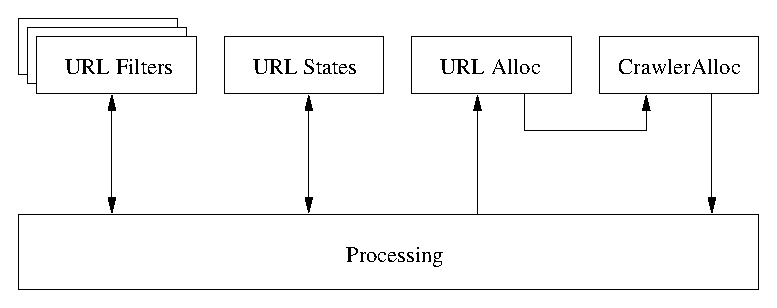
\epsfig{file=./images/disp_layers2.eps, scale=0.75}
  }
  \caption{Dispatcher crawling level components}
  \label{fig-disp_layers2}
\end{figure}

\subsection{URLFilters}
The URLFilter modules are responsible for ensuring that any URLs queued are allowed and within the current crawl domain. URLFilters are discussed further in Section \ref{sect-preventtrapped}. For their use in a production crawl, refer to Appendix \ref{appndx-config}.
\subsection{URLState}
Many papers\cite{ref1,ref2} mention using digests of URLs to minimise the size of the URLState table. Although Labrador's default URLState module does not, it would be straightforward to use a replacement that implements a Bloom filter, such as the Internet Archive crawler uses\cite{ref16}.\\
\ \\
The default URLState implemetation is just a light wrapper around a persistent hash table. Its purpose is to record which URLs are queued or have been fetchedand is used to prevent the crawler fetching any URL more than once.
\subsection{URLAlloc}
The URLAlloc module is responsible for enqueuing and dequeuing URLs onto the dispatchers master queue. Several different implementation exist - Breadth-First queuing, Depth-First queuing and Delay enqueing for Host Delay support. Breadth-first provides the best crawl results\cite{ref8}. Depth-first crawling is seldom used as it tends to become involved in the lower depths of a site before it finishes crawling the upper parts which are generally more important. The implementation of the Delay URLAlloc module (which queues in a breadth-first fashion) is described in Section \ref{sect-hostdelayimpls}. 
\subsection{CrawlerAlloc}
The CrawlerAlloc module is responsible for dequeuing URLs from the master queue then assigning and queuing them to a particular crawler, ready for that crawler's next request. If the crawler is running in partitioned mode, then the Partitioned CrawlerAlloc module must be used.

\section{Partitioning}\label{sect-partitioning}
\subsection{Overview}
To acheive scalable performance, Labrador was written as a distributed crawler, where the workload of fetching and processing URLs are performed by the crawler processes. Labrador has two modes for performing distributed crawling:
\begin{itemize}
\item{Simple\\} 
Simple mode means that each crawler will submit any URLs it found when processing a fetched page to the dispatcher and then ask the dispatcher for the next URL it had to fetch. This mode produces a processing burden on the dispatcher, due to the single threaded architecture used by the dispatcher, because the dispatcher can only process one command at a time. This means, when at high load, the dispatcher becomes the bottleneck for the entire crawling system.
\item{Partitioned\\}
Partitioned mode improves the speed of the system by allowing each crawler an amount of autonomy. Partitions of URLs are allocated to the each crawler and each crawler is permitted to crawl any URLs it finds that are in one of its partitions, without communication with the dispatcher. When a crawler discovers URLs not in its partition, then it submits them to the dispatcher for allocation.
\end{itemize}

\subsection{How Partitioning works}
Cho and Garcia-Molina describe\cite{ref3} three forms of partitioning a crawler: URL-hash based; Site-hash based; and Hierarchical. It should be noted that the URL-hash based forms, while discarded by Cho and Garcia-Molina, are effective in particular setups, such as crawling \{www,ir,www.brc\}.dcs.gla.ac.uk, where Host Delay is not required.\\
\\ \
When operating in partitioned mode, each of Labrador's crawlers, on receiving a URL, will compute the hash for that URL and allocate itself that hash. From then on, only URLs which have the same hash values as previously allocated URLs will be kept on the dispatcher. Others URLs, known as inter-partition links are sent back to the dispatcher for allocation, or to be given to the appropriate crawler if their partition is already allocated.\\
\\ \
Labrador operates as an exchanging crawler\cite{ref3}, which ensures that crawlers do not fetch pages from URLs that are not in its partition, thus nullifying any overlap between crawlers. However to keep optimal coverage, links are exchanged between crawlers via the distpacher. An alternative form, cross-over crawlers, allow crawlers to crawl URLs outwith their own partition, provided they have exhausted their own. In this form, without a high level of communication, there is a risk that different crawlers may fetch the same page. This uses excess resources and requires that the indexer is aware that it should skip URLs that have previously been processed. The final form of partitioned crawlers, firewalled crawlers, do not crawl out-with their own partitions and do not exchange links. This leads to poor coverage of the web, as parts of partitions may only be accessable from other partitions.

\subsection{Paritioning options}
I developed two main forms of partitioning crawls, based on URL-hash based and Site-hash based from above. Each form has several derivatives, as seen in Table \ref{tbl-partitions}.\\
\begin{table}
\begin{center}
\begin{tabular}{|l|l|l|l|}
\hline
\hline
\bf{No.}& \bf{Parition Name} & \bf{Type} & \bf{Supports Host Delay} \\
\hline
\hline
1 & SingleHostDirectory & URL-hash & No \\
\hline
2 & MultipleHostDirectory & URL-hash & No \\
\hline
3 & SingleHostTopDirectory & URL-hash & No \\
\hline
4 & MultipleHostTopDirectory & URL-hash & No \\
\hline
\hline
5 & SeenHost & Site-hash  & Yes \\
\hline
6 & DomainLevel & Site-hash & Yes \\
\hline
\end{tabular}
\caption{Labrador's Partition options}\label{tbl-partitions}
\end{center}
\end{table}

The Directory partition types assign different hash values to different directories, meaning that the crawling of any host could be split across several crawlers. This is why Host Delay is not supported for these Partition types.
\begin{itemize}
\item{SingleHostDirectory:}
This works by calculating the directory path to the file and using that as the hash value. This means that only files in the same directory are in the same partition.
\item{SingleHostTopDirectory:}
This partitioning scheme calculates the top level directory of the URL, so any files crawled in that directory or any subdirectory will be in the same partition.
\item{MultipleHostDirectory \& MultipleHostTopDirectory:}
These partitioning schemes are similar to their Single counterparts, except that the hostname of the URL is prepended to the hash value to ensure that the same directory path on a different host falls in a different partition.
\item{SeenHost:} This partitioning scheme works by ensuring that a crawler will only crawl URLs that have a hostname to which the crawler has been allocated before. URLs found that contain previously unseen hosts are returned to the disptacher.
\item{DomainLevel:} This is an extension of the SeenHost partitioning, where partitions are formed using levels of domain names. For instance, a crawler maybe assigned dcs.gla.ac.uk, while another is assigned arts.gla.ac.uk. This could be extended to form hierarchical crawling partitioning\cite{ref3}, where a master dispatcher may allocate a top-level domain, for instance .uk, to a local dispatcher, which will then further split .uk into smaller partitions to allocate to its crawlers.
\end{itemize}
Table \ref{tbl-partitionsex} gives examples of hash values calculated from sample URLs.
\begin{table}
\begin{center}
\begin{tabular}{|l|l|l|l|l|}
\hline
\bf{URL} & \bf{1} & \bf{3} & \bf{2} & \bf{4} \\
\hline
http://a/b/c/index.html & /b/c/ & /b/ & a/b/c/ & a/b/ \\
\hline
http://z/b/c/index.html & /b/c/ & /b/ & z/b/c/ & z/b/ \\
\hline
http://z/ & / & / & z/ & z/ \\
\hline
http://a/index.html & / & / & a/ & a/ \\
\hline
\end{tabular}
\caption{Hash values of example URLs under different partitioning schemes. URLs not having the same hash value in the set assigned to the crawler are sent to the dispatcher.}\label{tbl-partitionsex}
\end{center}
\end{table}
\ \\
Different alternatives of partitioning schemes may produce different amounts of inter-partition linkage. I evaluate different partitioning schemes in Section \ref{sect-evalpartitioning}.

\section{Crawler Architecture}
\subsection{Overview}
Labrador's crawlers use a layered approach to reduce cohesion between modules - many modules can be replaced by drop-in equivalents provided the same interface is implemented. The Agent module sits at the lowest level and performs all HTTP operations with remote hosts. It is tasked by the CrawlerHandler module, which also has event handlers that the Agent calls back to when the event occurs. The CrawlerHandler module passes the retrieved document to the ContentHandlers which save the content. The CrawlerHandler module also calls the currently loaded Manager module to obtain fresh URLs to be crawled. It is up to the implementor of the Manager module to perform communications with the dispatcher to retrieve the fresh URLs.\\

\begin{figure}[h]
  \centerline{
    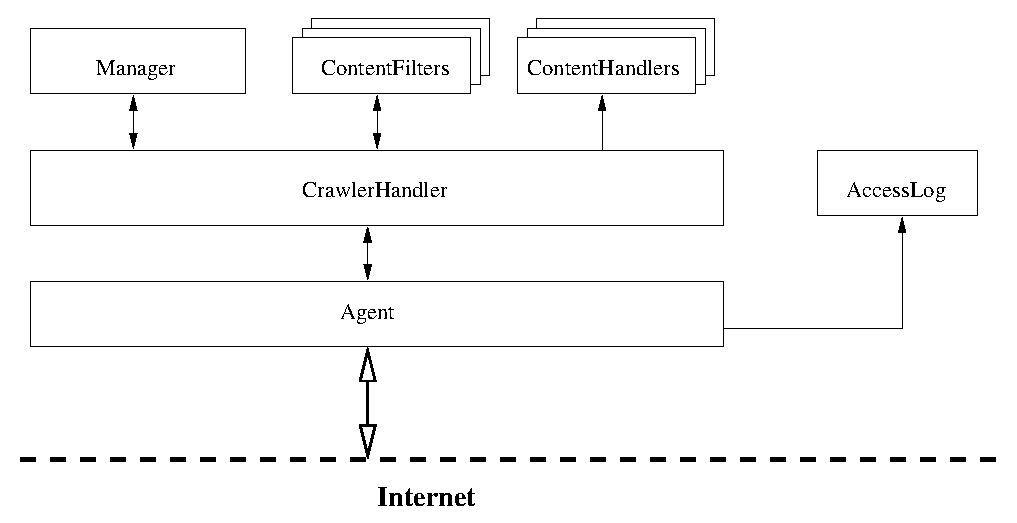
\epsfig{file=./images/crawler_layers.eps, scale=0.75}
   }
\label{fig-crawlerlayers}
\caption{Crawler architecture}
\end{figure}


\subsection{CrawlerHandler}
This is the centre of Labrador's crawler routines. The CrawlerHandler module basically executes a continuous loop, fetching a URL from the currently loaded Manager module and passing it to the Agent to crawl. When given a URL for a host it has not visited before, it will performs robots.txt checks, which may include a robots.txt fetch from the remote host.\\
\ \\
When the Agent finishes fetching a remote page, it calls the appropriate event method provided by the CrawlerHandler: agent\_success; agent\_redirect; agent\_failure. The agent\_success method is the most interesting, as it performs the most critical crawling tasks. Firstly it runs the document through any loaded ContentFilters. These will tell the crawler if it is permitted to follow any links or index the document. If the links can be followed, then any links are passed to the current Manager module. If the document can be indexed, then the document is passed to any loaded ContentHandlers.\\
\ \\
The agent\_redirect method handles redirects by requeuing the target URL of the redirect. The agent\_failure method simply informs the dispatcher that the URL failed. Both methods call event handlers in the ContentHandler modules in case any  wish to handle the redirect or failure cases.

\subsection{Agent}
The Agent module is responsible for lower-level network operations of the crawler (discounting dispatcher communications) and primarily exists to fetch URLs. When a URL is retrieved, the Agent calls the appropriate event handler in the CrawlerHandler, whether the event is a success, redirect or failure. In the case of a success, the Agent will pass back a Document object to represent the downloaded document.\\
\ \\
The libwww-perl modules from CPAN\cite{site1}, that the Labrador Agent uses for all underlying HTTP communications, are very powerful and mature, which keeps the source of the Agent module very clean. Labrador also makes full use of any HTTP extensions available to it. For instance, if the remote server supports HTTP compression, then Labrador will use it and decompress the content before handing to the Document object.\\
\ \\
While each Labrador crawler only supports fetching from one host at once, very little changes would have to be made to the rest of Labrador if the current Agent module was replaced by one which could support non-blocking socket fetches from multiple hosts concurrently. The current Agent implementation only opens one connection at once, and hence the the process is not downloading content while a finished page is being processed. The duration of time that a page is being processed would be ideal for the operating system to be downloading other pages for the same process. In practice, more than one crawler process is normally operating on any crawler machine at one time, and while one process is downloading, another is using the CPU to process a page. However, running multiple processes on one machine is not an optimial design, as each process requires separate memory space, and context switches become a significant overhead. For this reason many crawlers, such as Mercator\cite{ref2} and Googlebot\cite{ref7} use the non-blocking design, opening hundreds of connections per process, but only running one process per machine. Additionally, the disk I/O for saving crawled pages is serialized instead of being interspersed between competing processes, removing another overhead.\cite{book3}.

\subsection{ContentFilters}
The ContentFilters are a suite of modules that permits Labrador to note if a document can be indexed or its links followed. I have implemented five ContentFilter modules, described in Table \ref{tbl-contentfilters}.
\begin{center}
\begin{table}
\begin{tabular}{|l|l|}
\hline
\bf{Name} & \bf{Function} \\
\hline
Binary & Prevents binary content from being indexed. Terrier has no support for binary \\
& content and therefor it just pollutes the index. \\
\hline
ContentTypes & This ensures that Labrador only indexes the content that has a Content-type\\
& header that is desired. \\
\hline
FingerPrint & This is Labrador's duplicate detection module, which uses the MD5\cite{rfc1321}\\
& digest algorithm. This is further discussed in Section \ref{sect-dupdetection}.\\
\hline
MetaRobots & This module parses any meta-robots directives, as discussed in Section \ref{sect-metarobots}.\\
\hline
WhitelistLanguages & This module will let files through only if they contains at least one word \\
& from the specified stopword list. This simple technique is a good indicator\cite{wechsler97multilanguage} \\ & of language, but could be extended to cover all the techniques covered in the paper.\\
\hline
\end{tabular}
\caption{Labrador's ContentFilter modules}\label{tbl-contentfilters}
\end{table}
\end{center}

\subsection{Manager}
The Manager is one of two modules that have been specified to be loaded in the configuration file. These are Simple and Partitioned. \\
\ \\
The Simple module proxies requests from the CrawlerHandler straight to the dispatcher and has very little functionality itself.\\
\ \\
In contrast, the Partitioned Manager module actually replicates some of the functionality from the dispatcher. This is required, because a partitioned crawler has to function without constant communication with the dispatcher. The modules it shares with the dispatcher are: URLFilter, URLState, partitioning schemes and URLAlloc. Without these modules being available on the crawler, the partitioned crawler would not be as fully controlled as it would be under the Simple Manager module.

\subsection{Document handlers}
Document handlers are a suite of modules that handle any specific Content types that have special needs. Currently the types are HTML, Postscript, RTF and PDF files, although other classes could easily be written for say Microsoft Word or Powerpoint documents. The document handler for a type is responsible for converting the document, should it not be indexed in its current form (for instance PDF and Postscript documents), and performing link extraction on the type if possible.

\subsection{ContentHandlers}
Finally, the ContentHandler are the last link in the chain, where content is saved. Labrador has only been used to save documents for one indexer - the Terrier framework, so only one module has been developed here. The PreTerrier module saves the content in the way that exactly matches the needs of the Terrier indexer.

\section{Configuration File}
Although not particularly notable themseles, the Config module and the Labrador configuration file allow Labrador to be extremely flexible. Over the development of Labrador, I have matured a set of configuration files for specific crawls. To change a Labrador instance over to a different crawl, simply means specifying a different configuration file on the command line. As each crawler is started, it obtains its configuration file directly from the dispatcher - it has no need for a local copy of it. A sample configuration file is available in Appendix \ref{appndx-config}.\\
\ \\
When developing Labrador, the Config module was an early milestone, which meant that from then on any parameter that could be obtained from the configuration file was obtained, even if a default was set.
